\documentclass[aspectratio=169,11pt]{beamer}

\usetheme{default}
\usecolortheme{default}

% Minimal beamer: no navigation, no footline clutter
\setbeamertemplate{navigation symbols}{}
\setbeamertemplate{footline}[frame number]
\setbeamertemplate{frametitle}[default][left]
\setbeamertemplate{itemize items}[circle]
\setbeamertemplate{enumerate items}[default]

% Colors — nature-toned palette
\definecolor{charcoal}{HTML}{2C3E3A}       % deep forest, for titles
\definecolor{sage}{HTML}{5B7B6A}           % muted sage, for accents
\definecolor{clay}{HTML}{B07D62}           % warm clay, for emphasis
\definecolor{muted}{HTML}{8C8C8C}          % neutral gray, for footnotes
\definecolor{sand}{HTML}{F5F0EB}           % warm off-white, for callout boxes
\definecolor{darkred}{HTML}{9B4D3A}        % earthy red, for bias highlight

% Aliases for backward compat in body
\colorlet{navy}{charcoal}
\colorlet{accent}{sage}

\setbeamercolor{frametitle}{fg=charcoal}
\setbeamercolor{title}{fg=white}
\setbeamercolor{itemize item}{fg=sage}
\setbeamercolor{enumerate item}{fg=sage}
\setbeamercolor{normal text}{fg=charcoal}

% Fonts
\usefonttheme{professionalfonts}
\setbeamerfont{frametitle}{size=\large,series=\bfseries}
\setbeamerfont{title}{size=\Large,series=\bfseries}

% Packages
\usepackage{amsmath}
\usepackage{graphicx}
\usepackage{booktabs}
\usepackage{tikz}

% Metadata
\title{Can ML Recover Mechanism Design Propensity Scores?}
\subtitle{Cut 1 Results: Raw Mechanism Inputs}
\author{Anand Shah}
\date{March 2026}

\begin{document}

% =====================================================================
% TITLE
% =====================================================================
{
\setbeamercolor{background canvas}{bg=charcoal}
\begin{frame}[plain]
\vspace{2cm}
{\usebeamerfont{title}\usebeamercolor[fg]{title}\inserttitle}

\vspace{0.3cm}
{\color{clay}\hrule height 1.5pt}
\vspace{0.3cm}

{\color{white!80}\insertsubtitle}

\vspace{1.5cm}
{\color{white!60}\small\insertauthor\hspace{2cm}\insertdate}
\end{frame}
}

% =====================================================================
% SLIDE: What are we comparing?
% =====================================================================
\begin{frame}
\frametitle{If both $\hat{p}^{DA}$ and $\hat{p}^{ML}$ are correctly specified,
they should converge to the same object}

\begin{description}
\item[MDRD ($\hat{p}^{DA}$)] Analytic propensity scores from mechanism design theory.
Uses realized cutoffs, marginal priority, and MID.

\item[ML ($\hat{p}^{ML}_1$)] XGBoost trained to predict offer probabilities from raw
mechanism inputs.
No formula intermediates, no lottery numbers, no demographics.
\end{description}

\vspace{0.5cm}
\textbf{Cut 1 test:}
Both use only mechanism inputs (preferences, priorities, capacities, applicant pool).
If correctly specified, both estimate $P(\text{offer} \mid \text{type } \theta_i)$.

\vspace{0.5cm}
\begin{center}
\colorbox{sand}{%
\parbox{0.8\textwidth}{\centering\color{charcoal}\textbf{Result: They disagree.
Understanding why is the point of this talk.}}}
\end{center}
\end{frame}

% =====================================================================
% SLIDE: ML setup
% =====================================================================
\begin{frame}
\frametitle{XGBoost learns offer probabilities from four primitives:
preferences, priorities, capacities, and applicant pool}

\begin{columns}[T]
\begin{column}{0.48\textwidth}
\textbf{\color{accent}Model}
\begin{itemize}
\item XGBoost, 200 trees, learning rate 0.05
\item Max depth 6, early stopping (20 rounds)
\item 5-fold cross-fitting, grouped at student-year
\item 51,827 obs (ECE4, 2012--2020)
\item Offer rate = 50\%
\end{itemize}
\end{column}

\begin{column}{0.48\textwidth}
\textbf{\color{accent}Features (25, from primitives)}
\begin{itemize}
\item \textbf{Row:} priority, preference rank, capacity
\item \textbf{Student:} list length, best/worst priority above,
count of strong priorities above
\item \textbf{Bucket:} $n$ applicants, oversubscription ratio,
applicants by priority tier
\end{itemize}
\end{column}
\end{columns}

\vspace{0.5cm}
{\small\color{muted}\textit{No lottery numbers.
No MDRD intermediates (MID, cutoff, marginal priority).
No demographics.}}
\end{frame}

% =====================================================================
% SLIDE: Calibration
% =====================================================================
\begin{frame}
\frametitle{ML is well-calibrated; MDRD systematically underpredicts
for marginal students}

\begin{center}
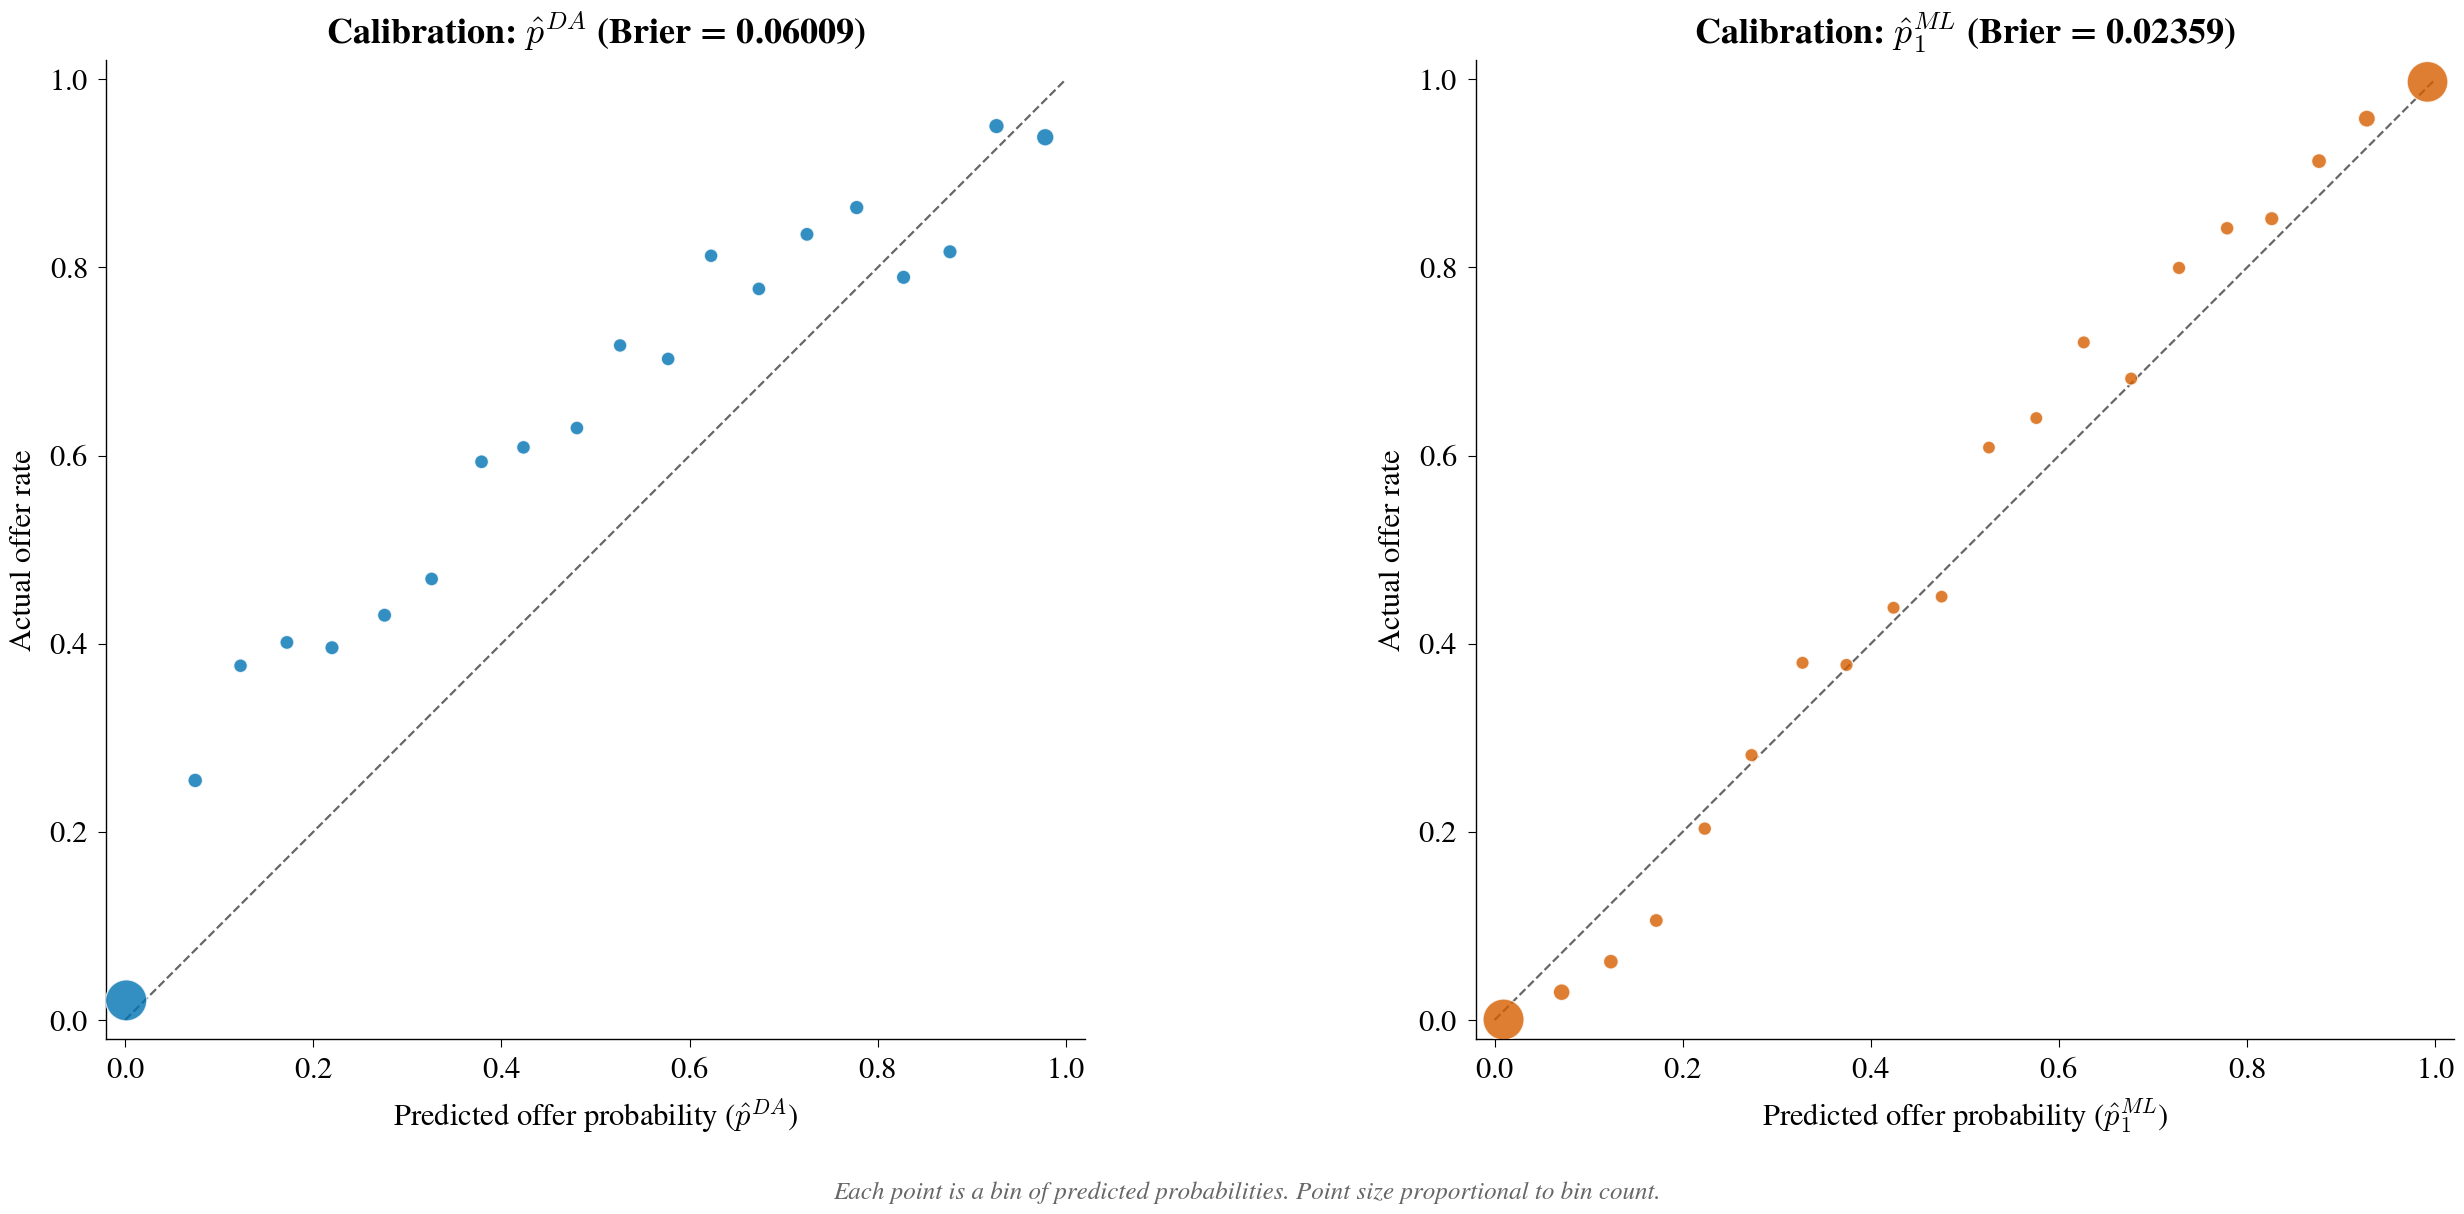
\includegraphics[width=0.92\textwidth]{figures/calibration.png}
\end{center}

\vspace{-0.3cm}
{\small\color{charcoal}\textbf{Brier score:}
$\hat{p}^{ML}_1 = 0.024$ vs $\hat{p}^{DA} = 0.060$.
ML is {\color{clay}2.5$\times$} more accurate.}
\end{frame}

% =====================================================================
% SLIDE: MSE by year
% =====================================================================
\begin{frame}
\frametitle{ML advantage is stable across years;
$\hat{p}^{DA}$ spikes in 2018 when the mechanism was redesigned}

\begin{center}
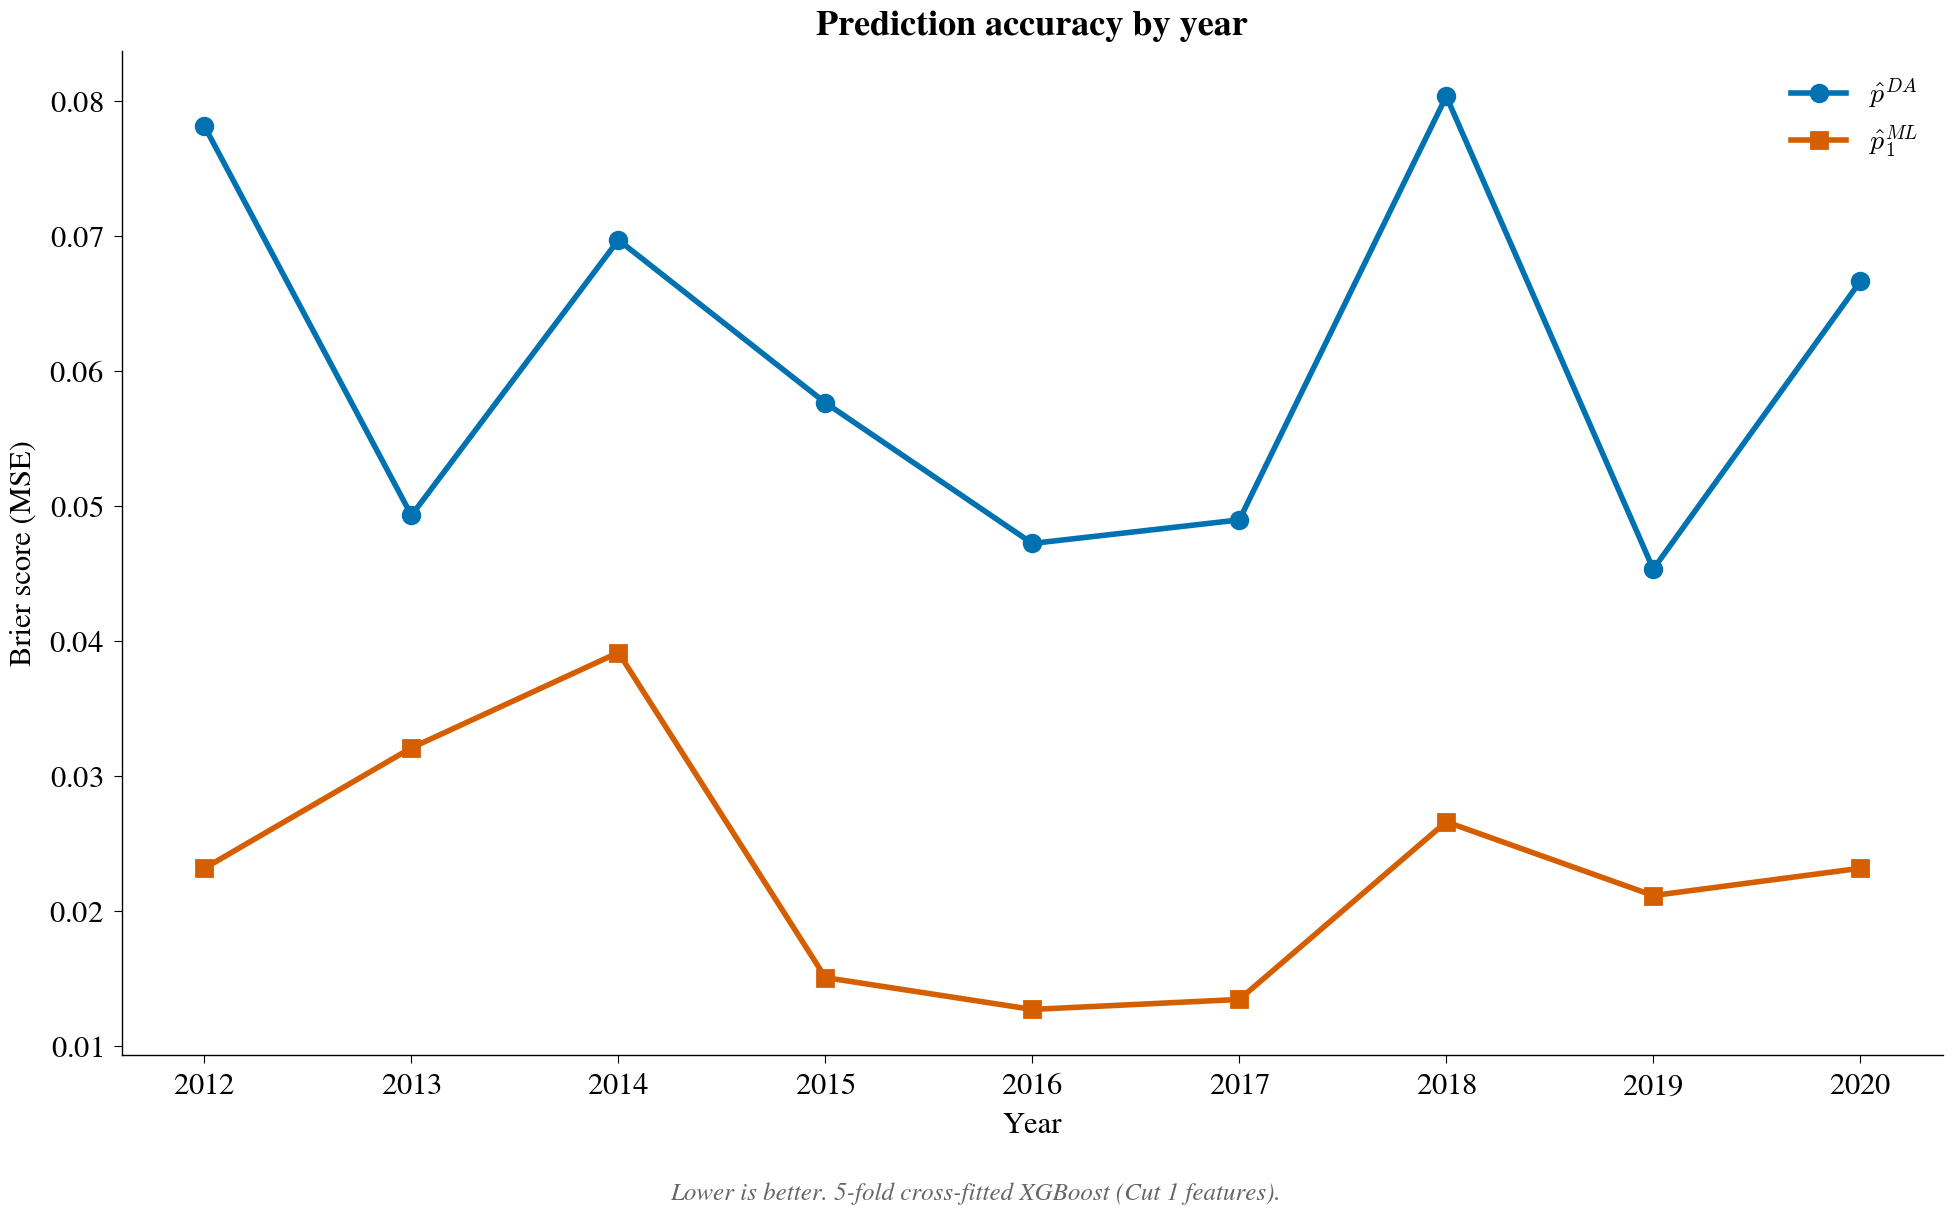
\includegraphics[width=0.75\textwidth]{figures/mse_by_year.png}
\end{center}

\vspace{-0.3cm}
{\small\color{muted}2018: programs consolidated from 214 to 132.
Priority tiers expanded.
ML adapts; formula does not.}
\end{frame}

% =====================================================================
% SLIDE: Feature importance
% =====================================================================
\begin{frame}
\frametitle{List length and competition---not priority or rank---are
the most informative features for ML}

\begin{center}
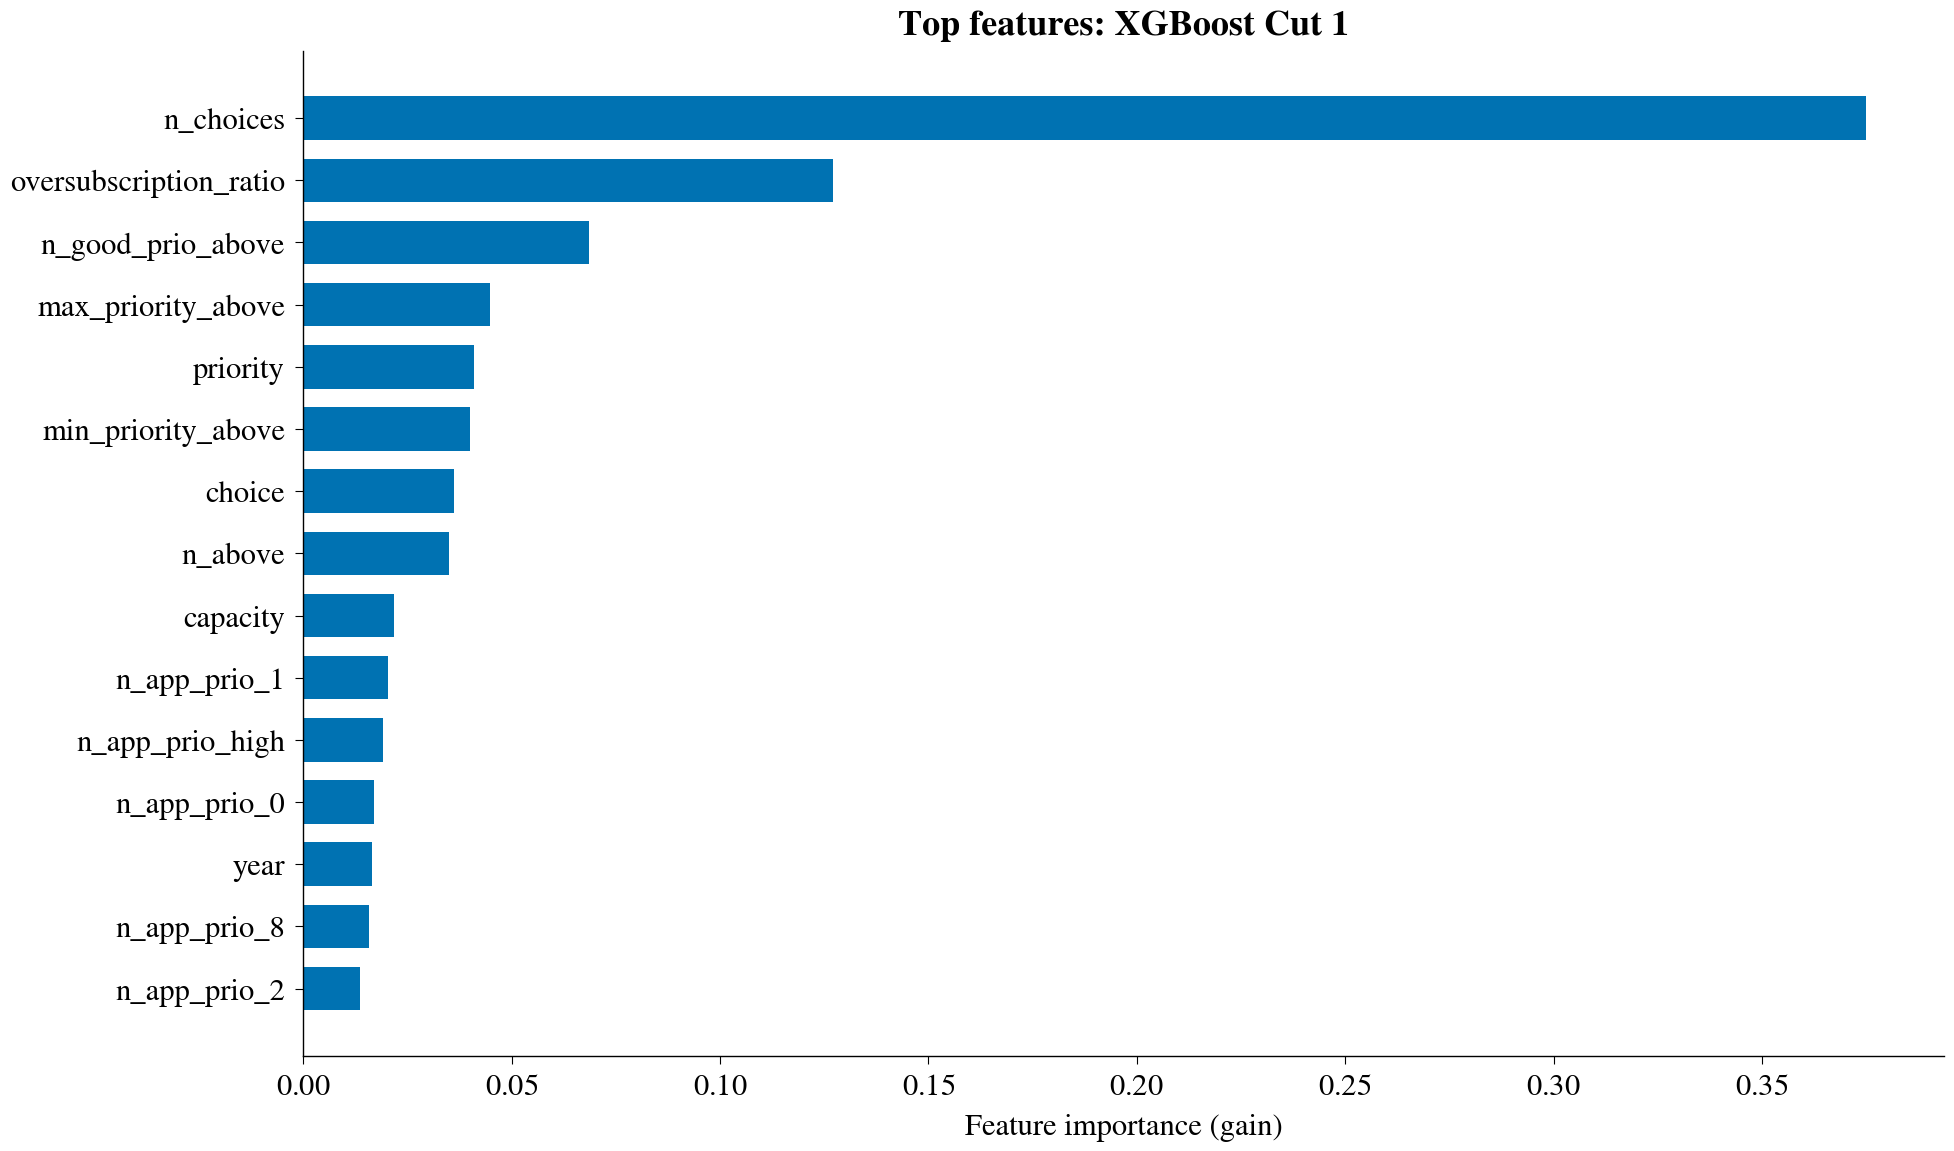
\includegraphics[width=0.75\textwidth]{figures/importance.png}
\end{center}

\vspace{-0.3cm}
{\small\color{muted}
\texttt{n\_choices} (37.5\%) captures how many ``bites at the apple''
a student has.
\texttt{oversubscription\_ratio} (12.7\%) captures market tightness.}
\end{frame}

% =====================================================================
% SLIDE: What explains the wedge --- diagnosis
% =====================================================================
\begin{frame}
\frametitle{The wedge comes from computing $\hat{p}^{DA}$ using realized
cutoffs from a single lottery draw}

\textbf{\color{accent}Current $\hat{p}^{DA}$ pipeline (from Stata code):}
\begin{enumerate}
\item Read realized marginal priority from who actually got offers
\item Read realized school cutoff from actual lottery numbers
\item Feed these single-draw objects into the MDRD formula
\end{enumerate}

\vspace{0.3cm}
This is a \textbf{plug-in estimator}, not a Monte Carlo DA probability.

\vspace{0.3cm}
The ``simulated'' pscores in the code also use a single simulated draw---same issue.

\vspace{0.5cm}
{\small\color{muted}\textit{Additional issues:
no status filtering (inflates $N$);
\texttt{lottery\_checker} computed but not acted on.}}
\end{frame}

% =====================================================================
% SLIDE: Why realized cutoffs bias downward
% =====================================================================
\begin{frame}
\frametitle{Realized cutoffs are order statistics that systematically
underestimate offer probabilities}

\begin{columns}[T]
\begin{column}{0.55\textwidth}
$N$ marginal applicants compete for $Q$ seats.

\vspace{0.3cm}
\textbf{\color{navy}True probability:} $\displaystyle\frac{Q}{N}$

{\small (symmetry: $Q$ winners from $N$)}

\vspace{0.3cm}
Realized cutoff $\hat\tau_s$ = $Q$-th order statistic of $N$ uniforms:
$$\mathbb{E}[\hat\tau_s] = \frac{Q}{N+1}$$

\vspace{0.2cm}
\textbf{\color{darkred}Bias} $= \displaystyle\frac{Q}{N} - \frac{Q}{N+1}
= \frac{Q}{N(N+1)}$

\vspace{0.2cm}
{\small\color{muted}\textit{Always positive. Largest in thin markets.}}
\end{column}

\begin{column}{0.42\textwidth}
\textbf{\color{accent}Examples}

\vspace{0.2cm}
\begin{tabular}{cccc}
\toprule
$N$ & $Q$ & True & Plug-in \\
\midrule
3 & 2 & 0.667 & 0.500 \\
5 & 3 & 0.600 & 0.500 \\
10 & 5 & 0.500 & 0.455 \\
100 & 50 & 0.500 & 0.495 \\
\bottomrule
\end{tabular}

\vspace{0.4cm}
\textbf{\color{accent}Empirical gradient}

\vspace{0.1cm}
{\small
\begin{tabular}{lr}
\toprule
$n_{\text{app}}$ & Bias \\
\midrule
$<10$ & $+0.31$ \\
$10$--$19$ & $+0.20$ \\
$20$--$39$ & $+0.17$ \\
$40$--$79$ & $+0.07$ \\
$80+$ & $+0.03$ \\
\bottomrule
\end{tabular}}
\end{column}
\end{columns}
\end{frame}

% =====================================================================
% SLIDE: Next steps
% =====================================================================
\begin{frame}
\frametitle{This week: recompute $\hat{p}^{DA}$ via full Monte Carlo,
then run Cut~2 with exhaust covariates}

\textbf{\color{accent}1.\quad Recompute $\hat{p}^{DA}$ via true rerandomization}

Fix primitives (preferences, priorities, capacities).
Redraw all lottery numbers.
Run full DA.
Record offers.
Average over 1{,}000+ draws.
$\hat{p} = \overline{\text{offer}}$ across draws.

\vspace{0.5cm}
\textbf{\color{accent}2.\quad Verify $\hat{p}^{DA}_{\text{new}} \approx \hat{p}^{ML}_1$}

If the corrected DA scores match ML predictions,
the formula was the problem and ML has been recovering the correct
object all along.

\vspace{0.5cm}
\textbf{\color{accent}3.\quad Run Cut 2: add exhaust covariates}

Add demographics, neighborhood, school characteristics.
If $\hat{p}^{ML}_2 > \hat{p}^{ML}_1$,
exhaust covariates carry information about selection beyond
mechanism inputs.
This is the substantive test.
\end{frame}

\end{document}
